\subsection{Efficiency}
\label{sec:systems}

At 224 pixels, \mn{} passes 392 rather than 784 patches to the latent
stage and requires an estimated 14.13 GMAC per image, compared with
22.41 GMAC for dense DeiT-S/8, a 37.0\% reduction. The estimate excludes
indexing and data movement; Table~\ref{tab:a100-efficiency} measures their
combined effect with the rest of the implementation on an A100.

Compilation lowers the measured \mn{} batch-64 latency from
36.30 to 27.24\,ms, a 25.0\% reduction on the tested A100 configuration.
Compiled ToMe takes 27.22\,ms; peak allocated memory is 0.627\,GiB
for \mn{} and 0.614\,GiB for ToMe. Table~\ref{tab:a100-efficiency}
and Figure~\ref{fig:a100-efficiency} report both execution modes.
These model-only benchmarks use random weights and synthetic inputs;
Appendix~\ref{app:followup} specifies the measurement and compilation settings.

\begin{table}[H]
\caption{Synthetic A100 inference at 224 pixels with fp16 autocast
and random weights. B1/B64 denote batch sizes 1 and 64; memory is
batch-64 peak allocated and reserved GiB. The eager \mn{} B1 range
spans two independent run medians.}
\label{tab:a100-efficiency}
\centering\footnotesize
\setlength{\tabcolsep}{3.5pt}
\begin{tabular}{lrr}
\toprule
Model & 224 px (ms) & 384 px (ms) \\
\midrule
Dense DeiT-S/8 & 30.09 & 109.43 \\
ToMe, proportional attention on & 34.42 & 133.36 \\
ToMe, proportional attention off & 29.71 & 96.05 \\
MergeNet $R=3$ & 49.16 & 144.97 \\
MergeNet $R=3$, BNHD & 46.56 & 138.11 \\
MergeNet $R=5.143$ & -- & 218.25 \\
MergeNet $R=5.143$, BNHD & -- & 211.40 \\
\bottomrule
\end{tabular}

\end{table}

\begin{figure}[H]
\centering
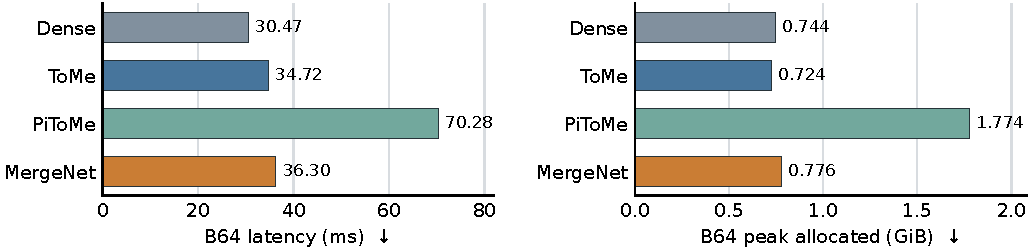
\includegraphics[width=\linewidth]{figures/a100_efficiency.pdf}
\caption{Batch-64 A100 inference with random weights.
Solid bars denote eager execution; hatched bars denote compiled execution.
Latency and peak allocated memory use the measurements in
Table~\ref{tab:a100-efficiency}; lower is better.}
\label{fig:a100-efficiency}
\end{figure}

A separate high-resolution benchmark on an H20 measures 136.54\,ms
for \mn{} and 170.61\,ms for dense DeiT-S/8 at 384 pixels and batch 64.
Peak allocated memory is 2.969 and 1.983\,GiB, respectively.
This operating point illustrates a latency reduction alongside a larger
memory footprint. Appendix~\ref{app:highres-efficiency} reports the
training and inference measurements under that hardware setup.
